\chapter{L'oscillateur de Van der Pol}

L'equation de Duffing forcé
On s'interesse à l'équation de Van der Pol. Qui fut crée en --- par Van der Pol pour modeliser un certain phénomène.
\begin{equation}
    \ddot{x} + x + \epsilon(x^2 - 1)\dot{x} = 0
    \label{eq:vdp}
\end{equation}
C'est un système non conservative avec une particuliarité intéressente. 
Le signe du terme d'ammortissement $\epsilon(x^2 - 1)\dot{x}$ change en fonction... 
Lorsque $|x|<1$, le coefficient d'ammortissement négatif fournit de l'énergie au système et dans le cas contraire $|x|>1$, il en dissipe. 
Ce comportement particulier donne lieu a des oscillations entretenue de manière autonome.

\begin{comment}
\begin{figure}[!t]
    \begin{subcaptionblock}{.47\linewidth}
      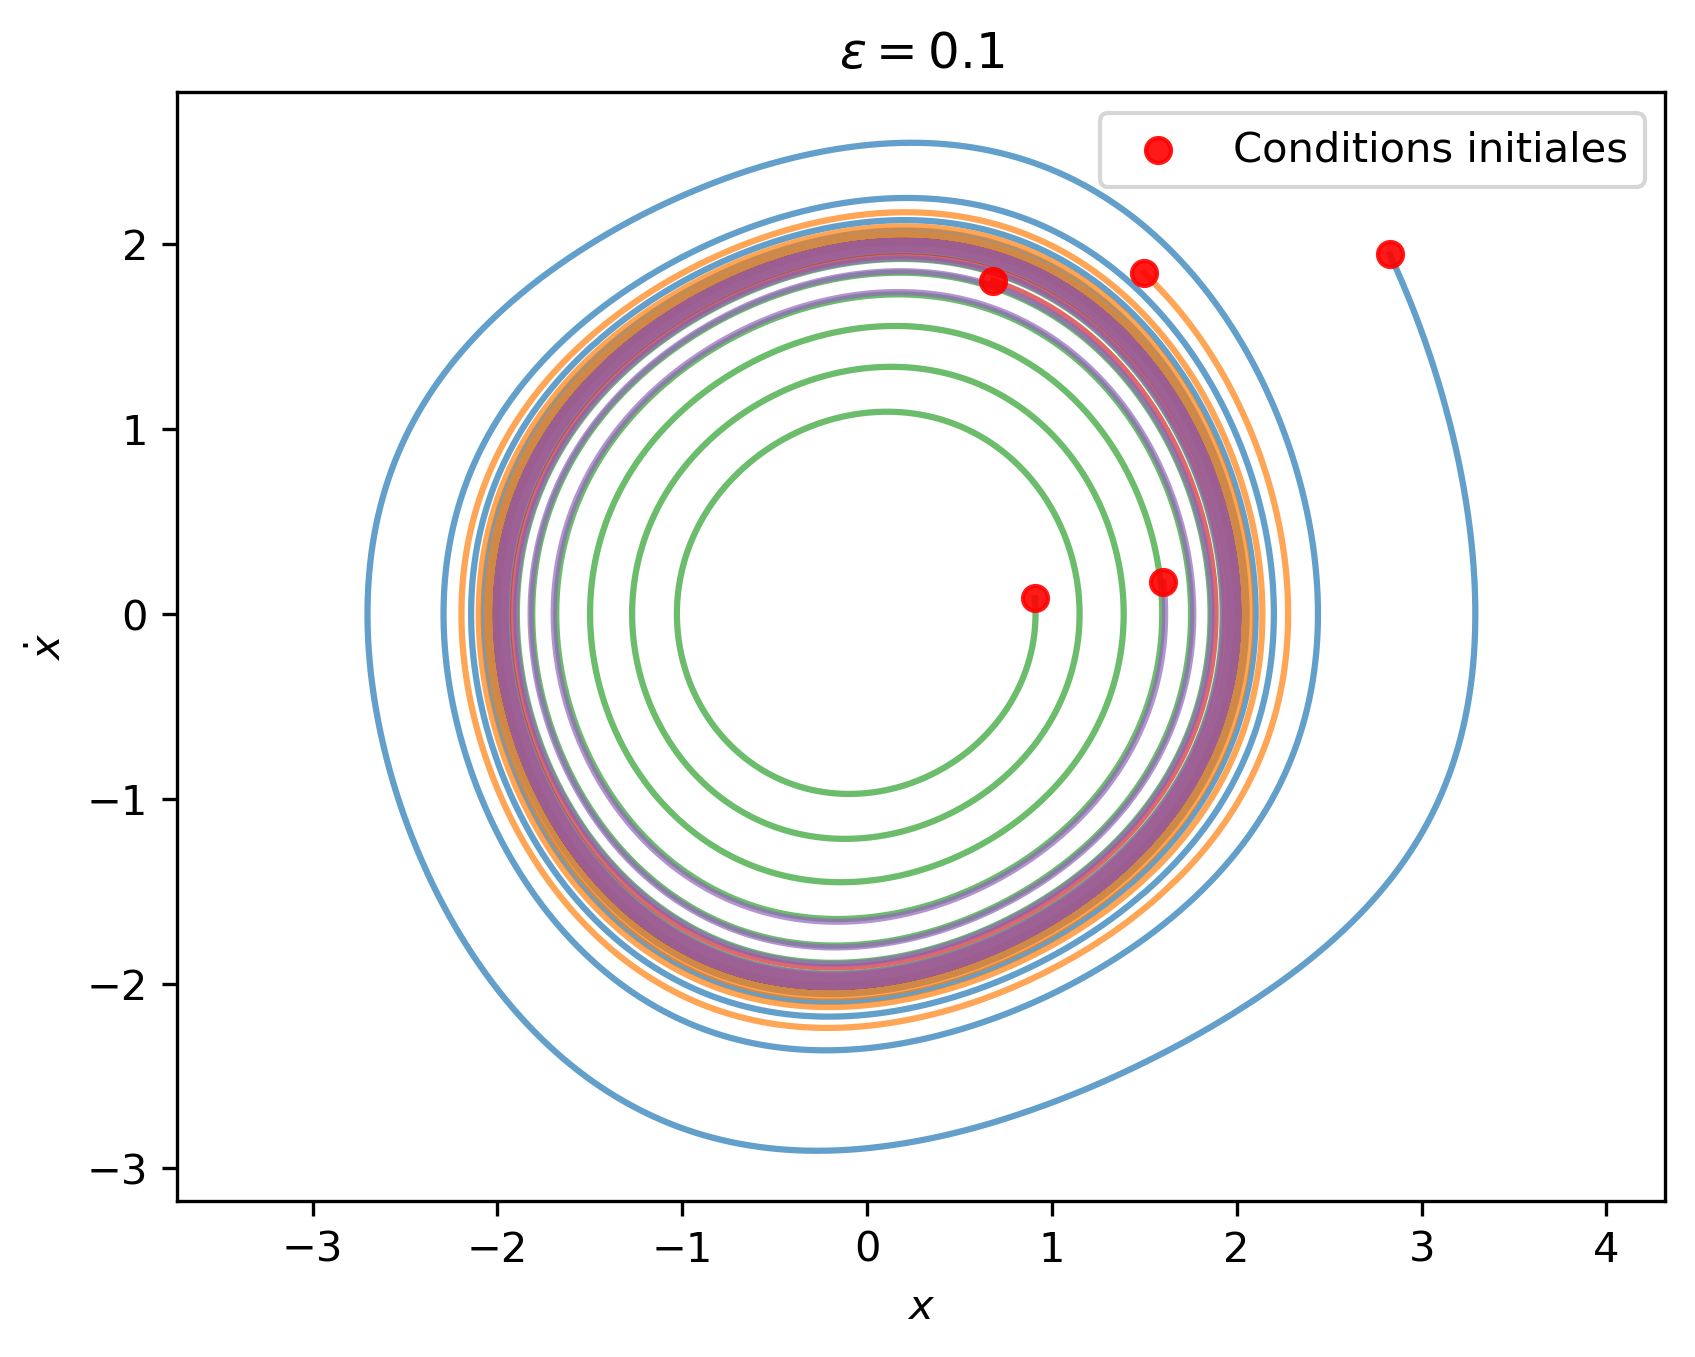
\includegraphics[width=\linewidth]{images/vdp/vanderpol_small.png}%
      \phantomcaption
    \end{subcaptionblock}
    \hfill
    \begin{subcaptionblock}{.47\linewidth}
      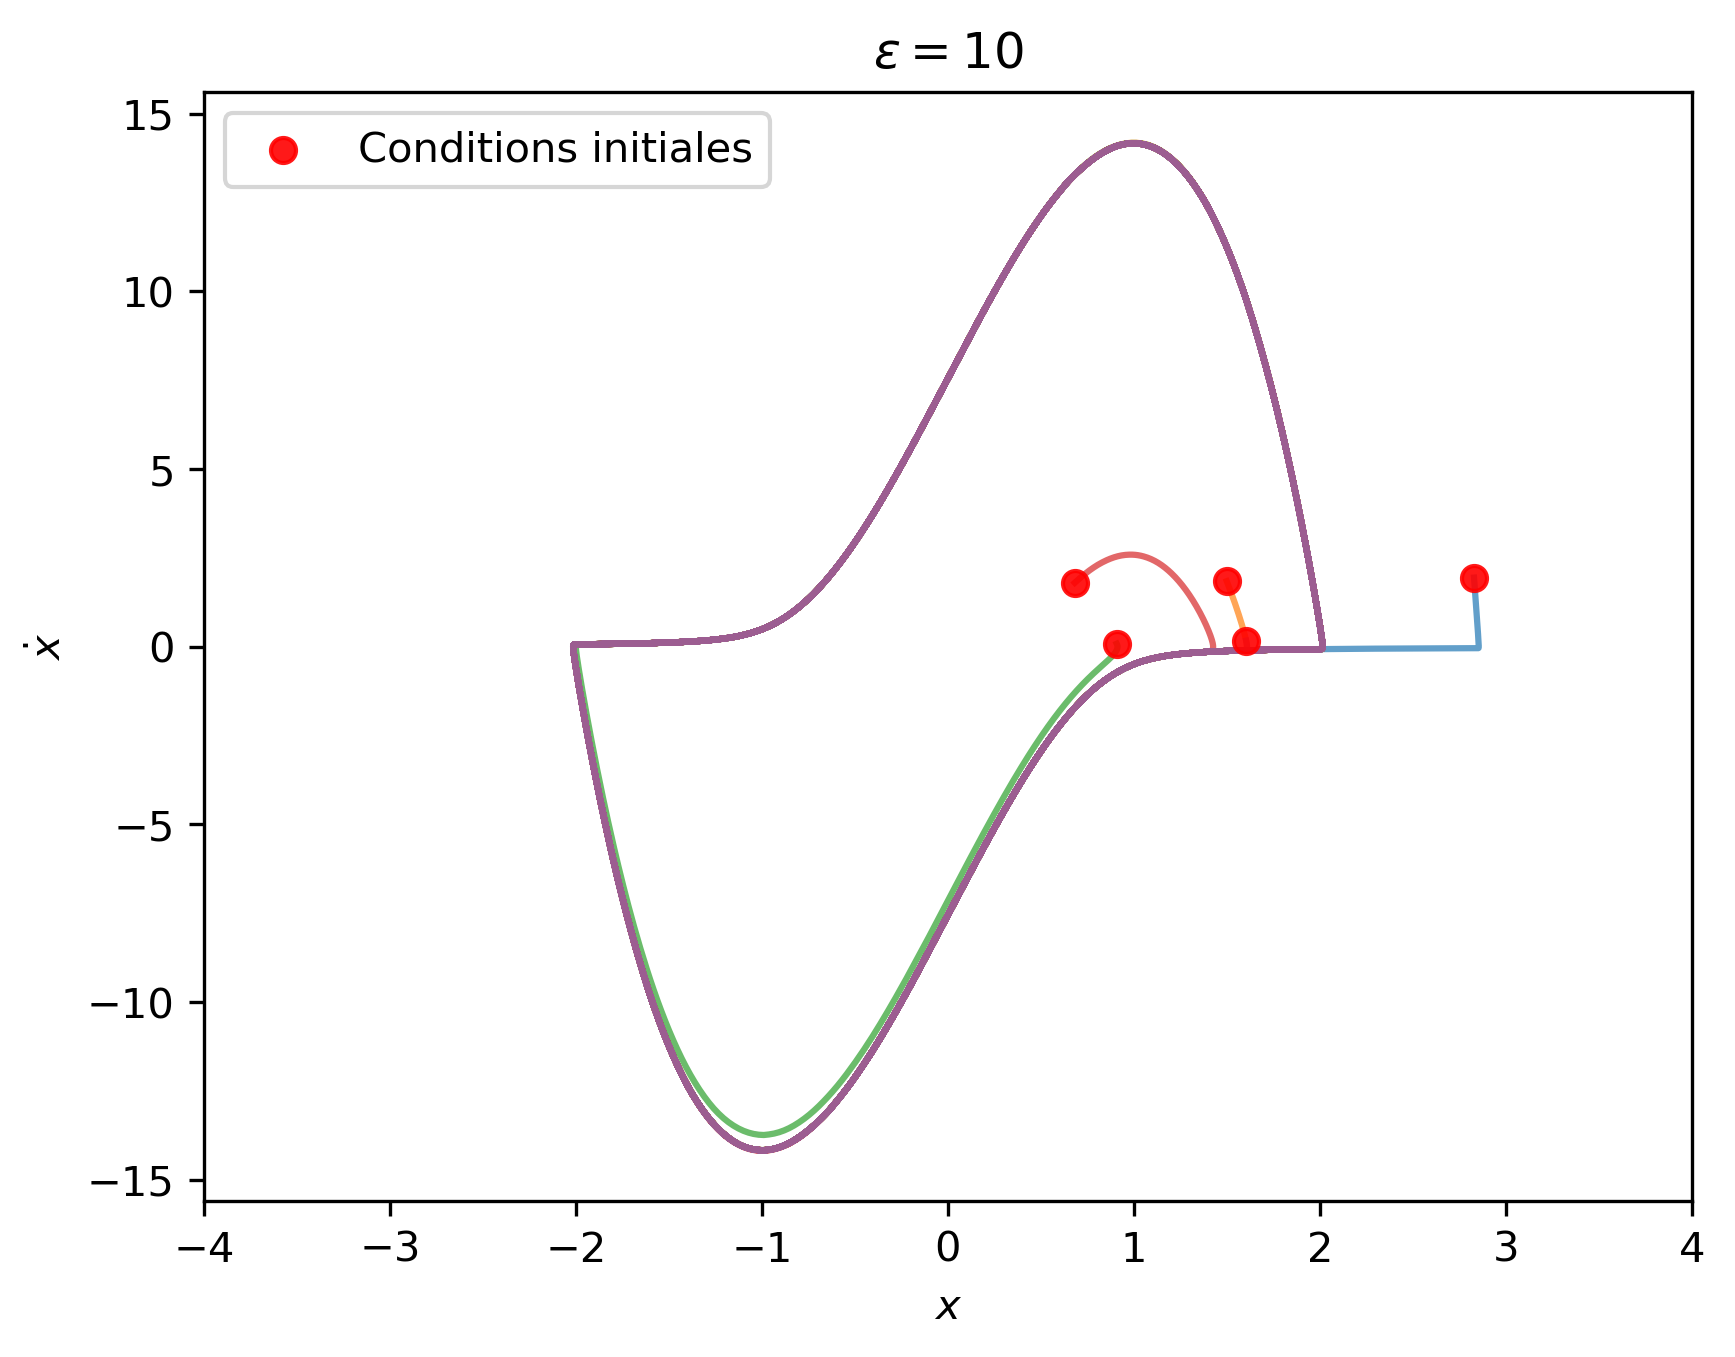
\includegraphics[width=\linewidth]{images/vdp/vanderpol_large.png}%
      \phantomcaption
    \end{subcaptionblock}
    \label{fig:portrait_vdp}
    \caption{Portraits de phase de l'oscillateur Van der Pol obtenu par intégration numérique pour faible et grand $\epsilon$, conditions initiales aléatoires}
\end{figure}
\end{comment}

\begin{figure}[t]
    \begin{subcaptionblock}{\linewidth}
        %\hfill
        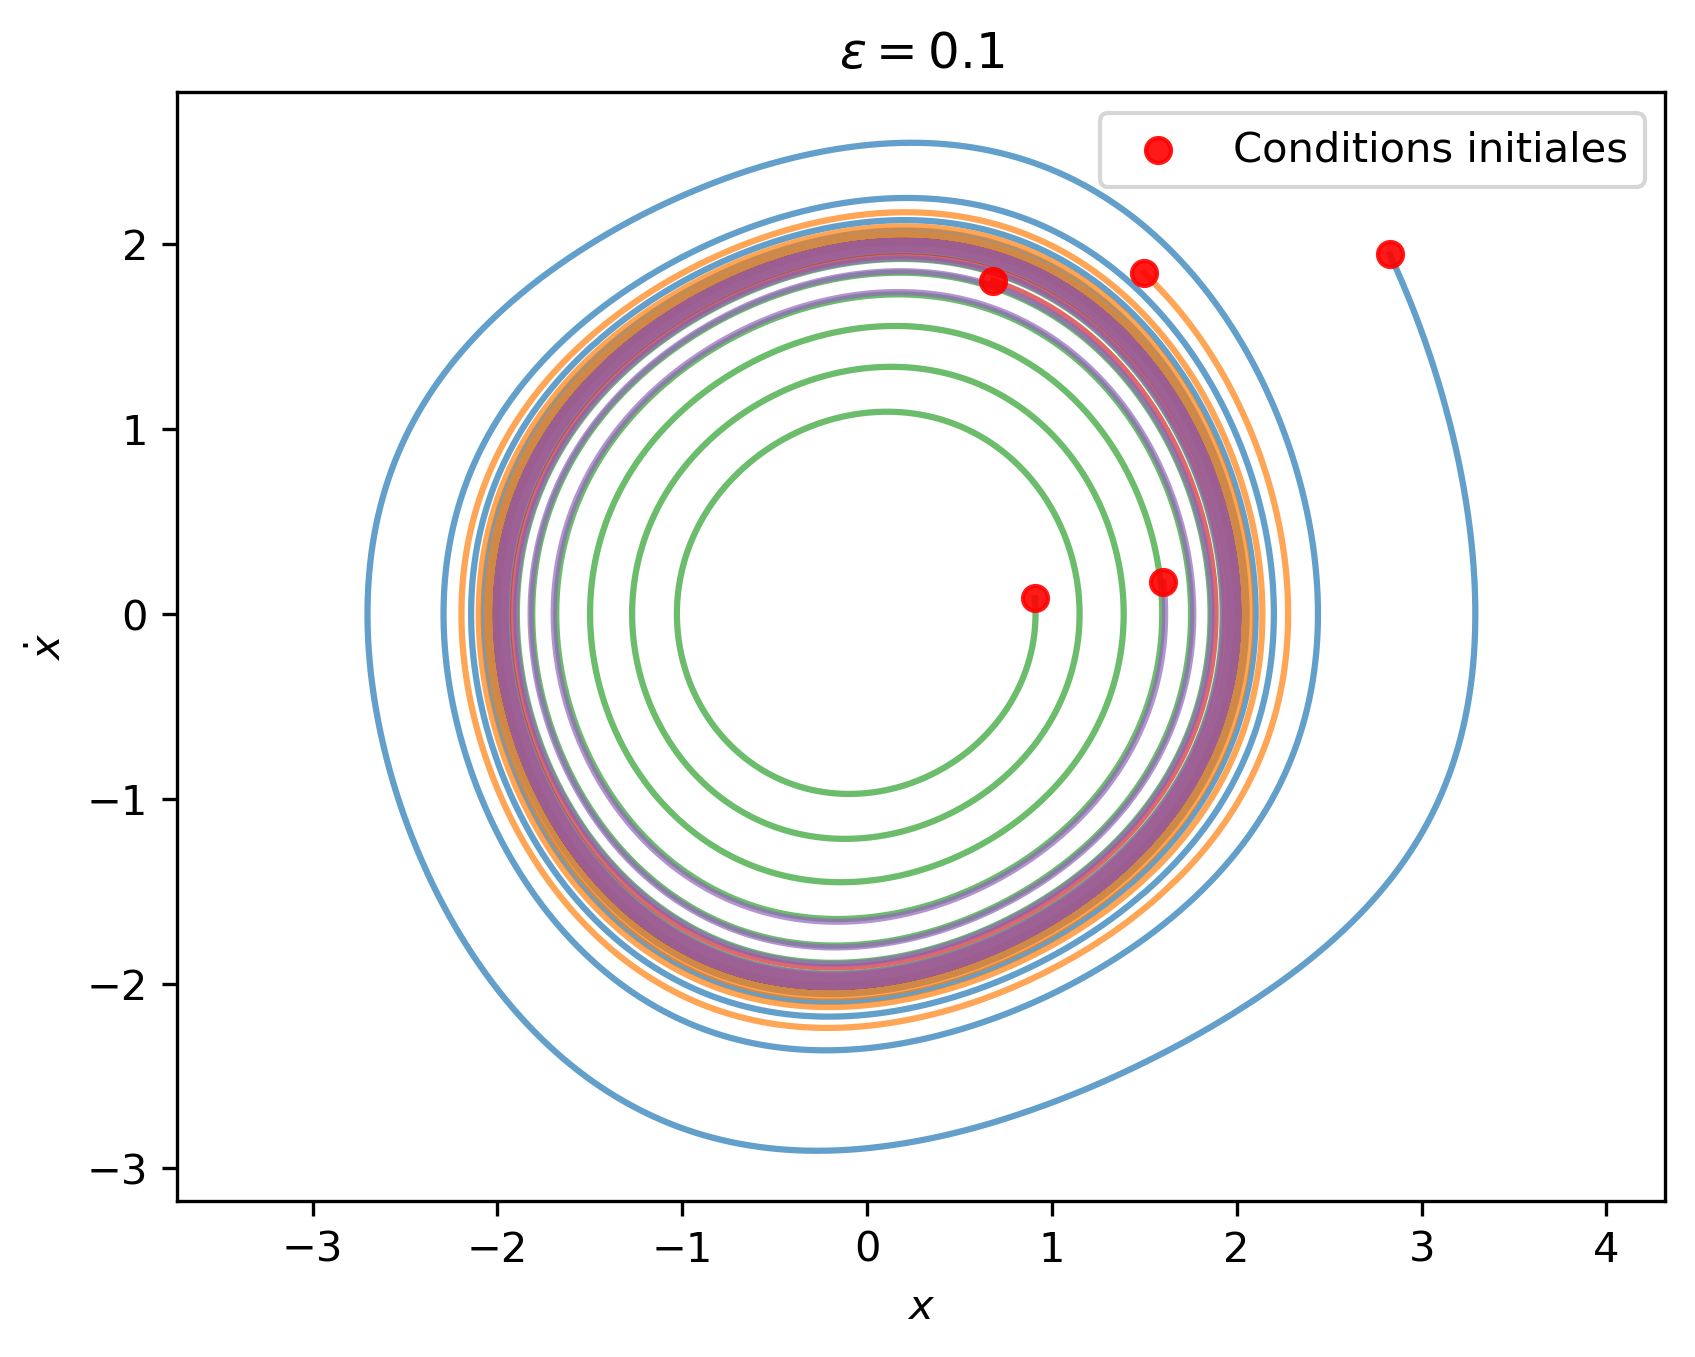
\includegraphics[width=.45\linewidth]{images/vdp/vanderpol_small.png}%
        \hfill
        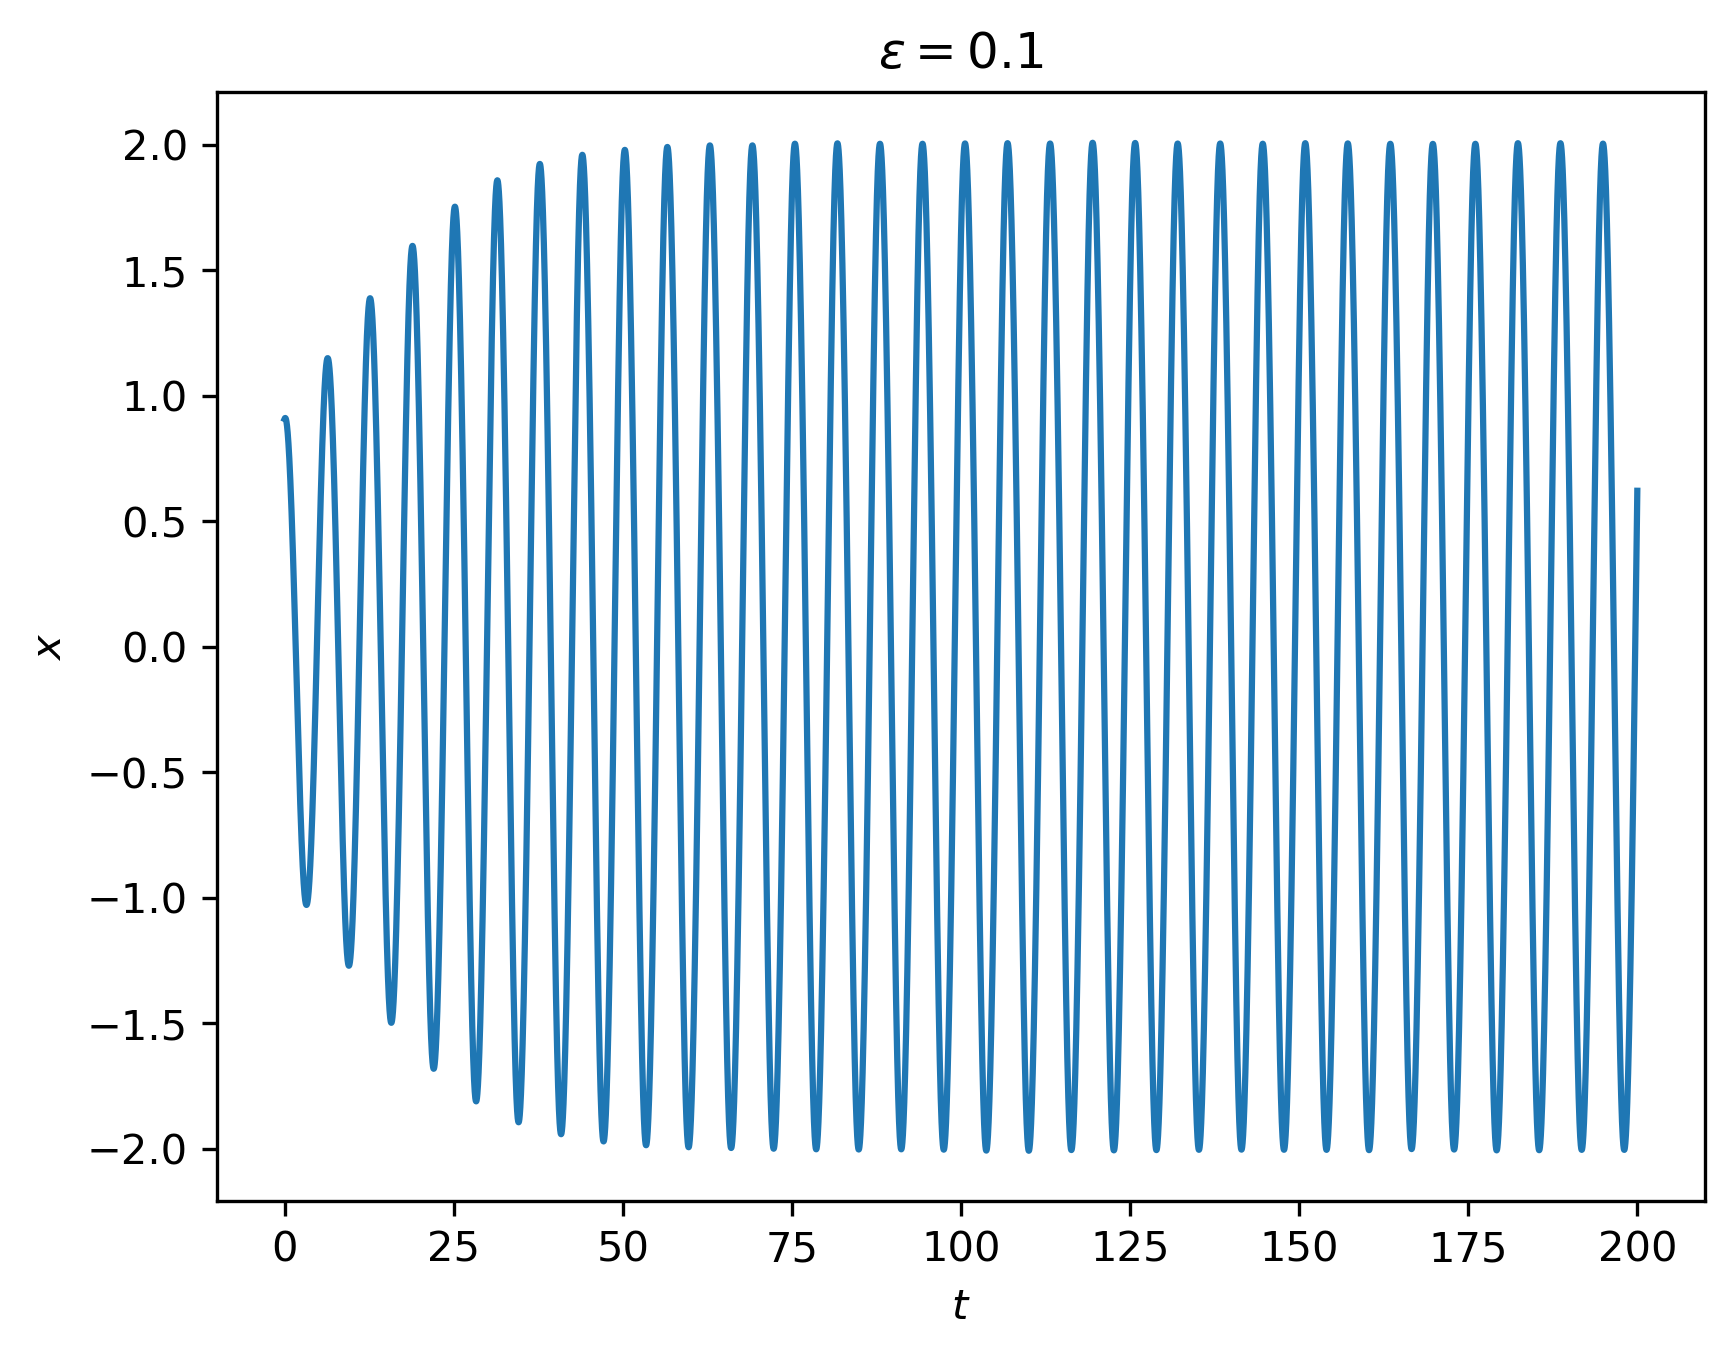
\includegraphics[width=.45\linewidth]{images/vdp/vanderpol_small_x.png}%
        %\hfill
        %\centering
        %\caption{$\epsilon = 0.1$}
    \end{subcaptionblock}
    %\hfill
    \begin{subcaptionblock}{\linewidth}
        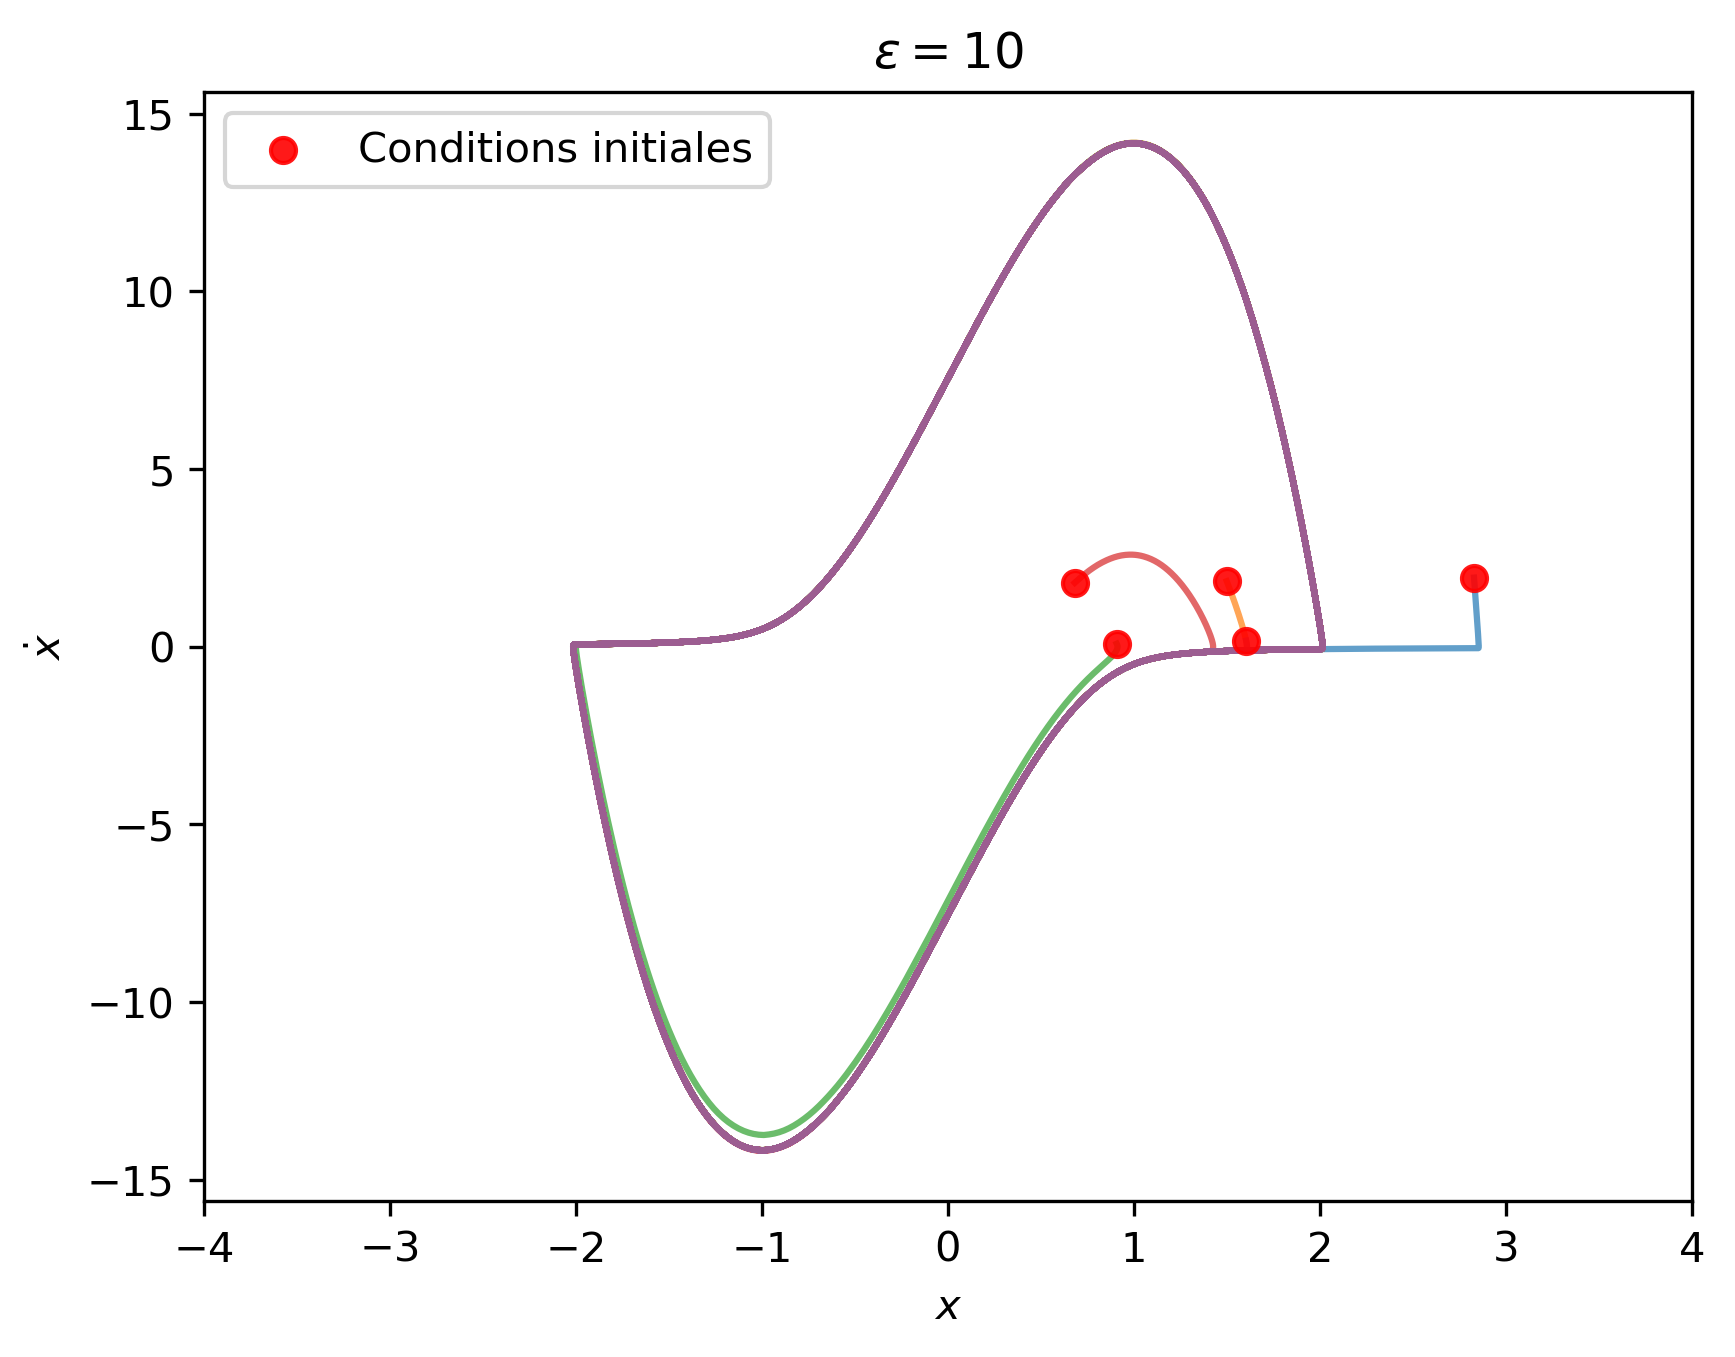
\includegraphics[width=.45\linewidth]{images/vdp/vanderpol_large.png}%
        \hfill
        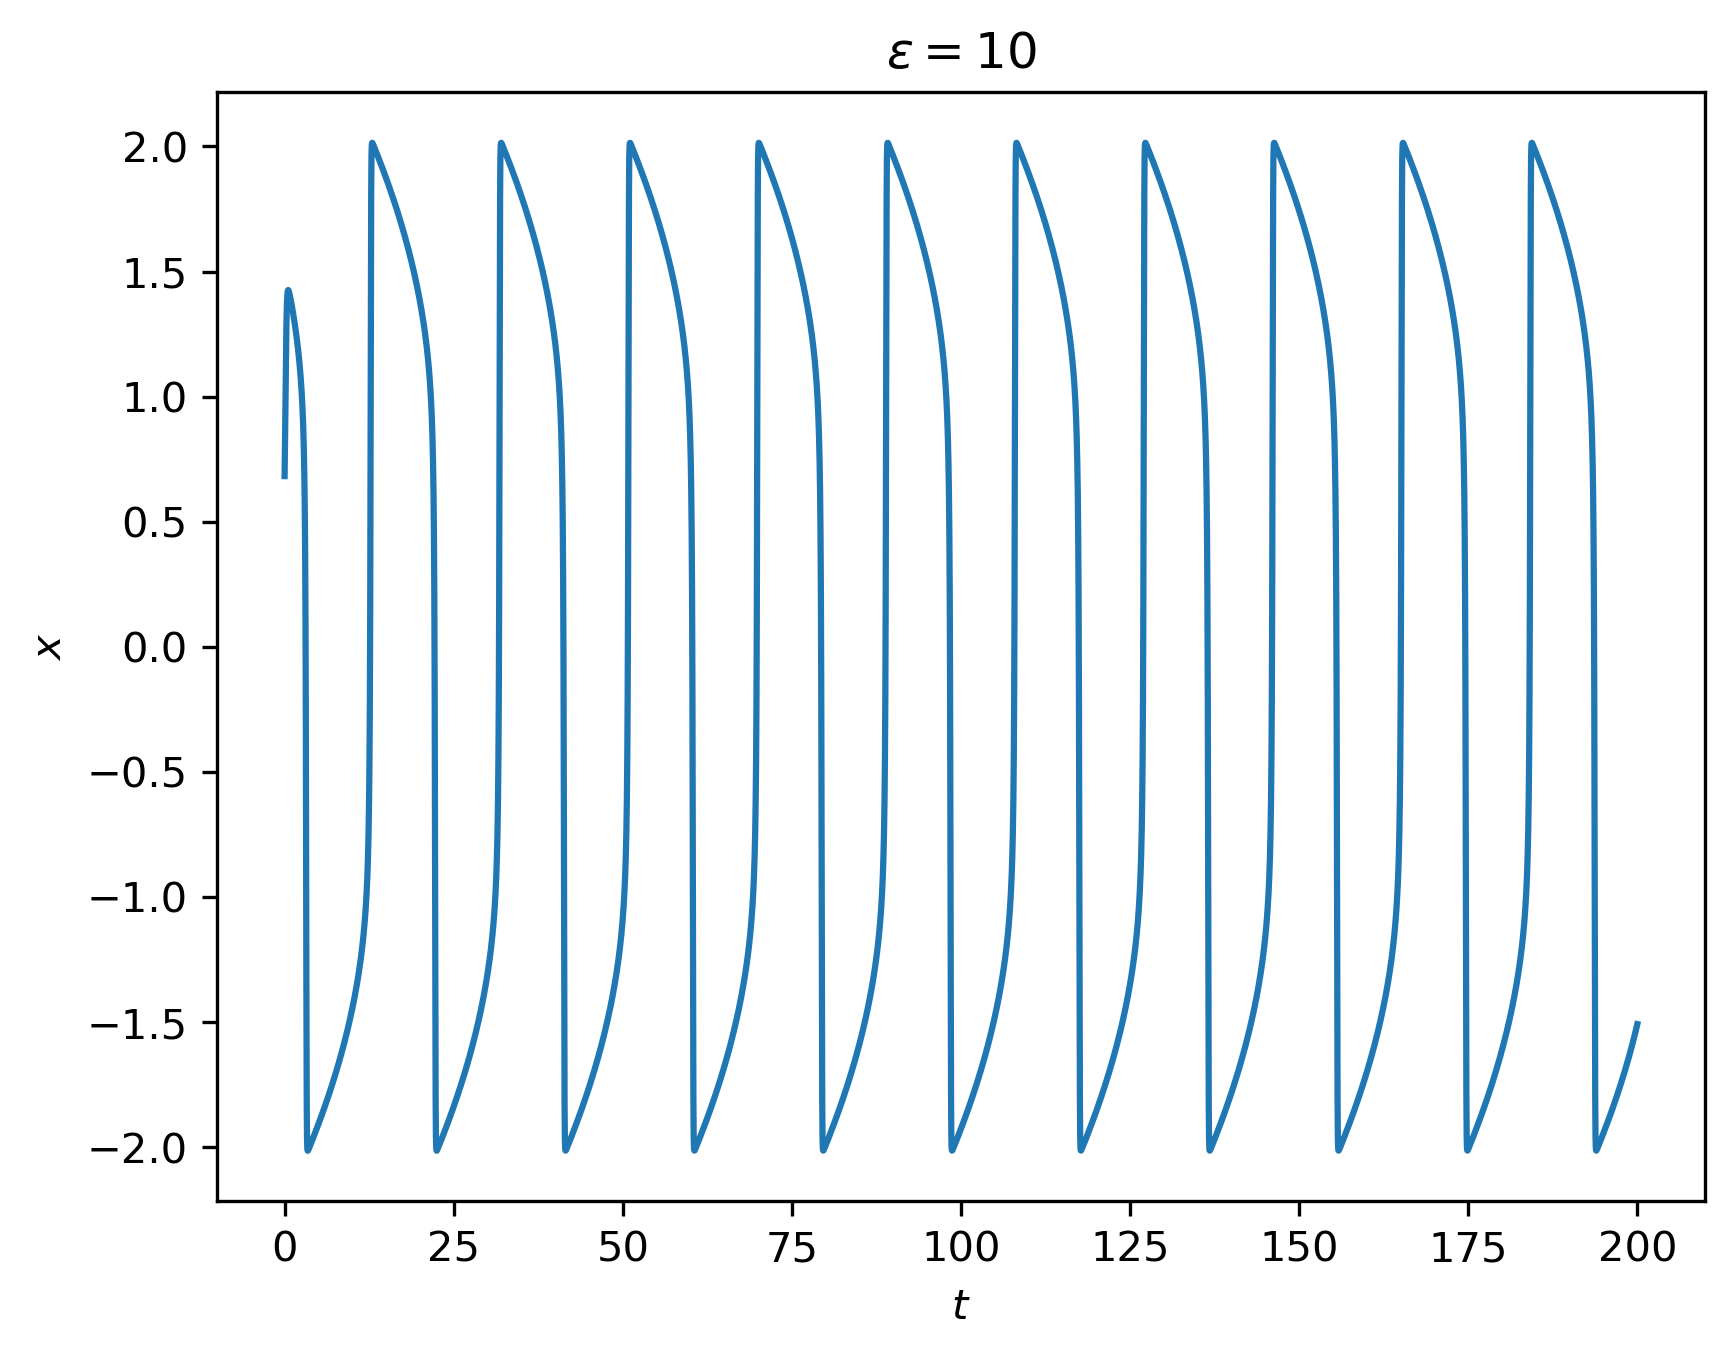
\includegraphics[width=.45\linewidth]{images/vdp/vanderpol_large_x.png}%
        %\caption{$\epsilon = 5$}
    \end{subcaptionblock}
    \label{fig:portrait_vdp}
    \caption{Portraits de phase de l'oscillateur Van der Pol obtenu par intégration numérique pour faible et grand $\epsilon$, conditions initiales aléatoires}
\end{figure}


Avec une étude numérique du système sur le plan de phase, on constate que le système tend vers une unique orbite isolée, quelles que soient les conditions initiales imposées. 
Une telle orbite dans l'espace de phase s'appelle un \emph{cycle limite}. On voit notamment que pour petit $\epsilon$, que le cycle limite est fortement elliptique avec des oscillations quasi-circulaire, 
alors que pour grand $\epsilon$ le cycle est fortement déformé et caractérisé par des oscillations de relaxations.
%c'est une oscillation de relaxation a cause des 
%De ce fait, il est possible de faire une analyse énergetique rudimentaire du système, en supposant que 

En comparent les oscillations des système faiblement et fortement non-linéaire, on observe aussi que la fréquence d'oscillation diverge de la fréquence naturelle $\omega_0 = 1$ lorsque $\epsilon$ augmente. 
%Cette remarque, faite en premier par Lindstedt, va nous inspirer à chercher une solution approximative de \eqref{eq:vdp} sous forme d'un development perturbative
On va chercher une solution approximative de \eqref{eq:vdp} sous forme d'un development perturbative. En particulier, on va utiliser la méthode de Lindstedt, 
qui nous permet de prendre en compte la dépendence qu'a $\epsilon$ sur la fréquence d'oscillations. L'approche consiste à définir une echelle de temps normalisé et de prendre la fréquence $\omega$ du cycle limite comme étant un inconnu qui dépend de $\epsilon$ :
\begin{equation}
    \tau = \omega(\epsilon)t
    \qquad
    \omega(\epsilon) = \omega_0 + \epsilon\omega_1 + \epsilon^2\omega_2 + O(\epsilon^3)
\end{equation}
La justification derrière cette transformation d'echelle de temps est qu'elle nous permet de définir $x(\tau)$ comme étant $2\pi$ periodique, 
alors que $x(t)$ à une periode qui nous est inconnue en raison de sa dépendence sur $\omega$.

\begin{equation}
    x(t, \epsilon) = x_0(t) + \epsilon x_1(t) + \epsilon^2 x_2(t) + O(\epsilon^3)
\end{equation}


Notre hypothèse de départ étant que la fréquence $\omega$ du cycle limite est un inconnue qui dépend de $\epsilon$, 
ce qui fait que $x(t)$ à une periode qui elle aussi est inconnue. 
En changeant d'échelle de temps, on peut 

dépend de $\epsilon$, la solution $x(t)$ aura donc une période qui lui aussi dépend de $\epsilon$. Or, on aimerai trouver un solution


